\documentclass[11pt,a4paper,sans]{moderncv} % Font sizes: 10, 11, or 12; paper sizes: a4paper, letterpaper, a5paper, legalpaper, executivepaper or landscape; font families: sans or roman
% \usepackage{nopageno}

\moderncvstyle{casual} % CV theme - options include: 'casual' (default), 'classic', 'oldstyle' and 'banking'
\moderncvcolor{blue} % CV color - options include: 'blue' (default), 'orange', 'green', 'red', 'purple', 'grey' and 'black'
\usepackage{lipsum} % Used for inserting dummy 'Lorem ipsum' text into the template
\usepackage{multicol}
\usepackage{url}
%\usepackage{graphicx} %for signature
\usepackage[english,ngerman]{babel}
\usepackage{datetime}
\usepackage{array,booktabs,makecell}
\renewcommand\theadfont{\bfseries}% bold tabular headers
\renewcommand\theadalign{cc}% centred tabular headers
\renewcommand\theadgape{}% booktabs rules already add vertical spacing
\newcommand{\head}[1]{\textnormal{\textbf{#1}}}

\def\Plus{\texttt{+}}
\def\Minus{\texttt{-}}
\newcommand{\quotes}[1]{``#1''}

\usepackage[scale=0.85, left=1.2cm, right=1.2cm]{geometry} % Reduce document margins
\setlength{\hintscolumnwidth}{45mm} % Uncomment to change the width of the dates column
%\setlength{\makecvtitlenamewidth}{10cm} % For the 'classic' style, uncomment to adjust the width of the space allocated to your name
\usepackage{ragged2e}


\newcommand{\cvdoublecolumn}[2]{%
	\cvline{}{%
		\begin{minipage}[t]{\listdoubleitemmaincolumnwidth}#1\end{minipage}%
		\hfill%
		\begin{minipage}[t]{\listdoubleitemmaincolumnwidth}#2\end{minipage}%
	}%
}

\newcommand{\cvreference}[7]{%
	\textbf{#1}\newline% Name
	\ifthenelse{\equal{#2}{}}{}{\addresssymbol~#2\newline}%
	\ifthenelse{\equal{#3}{}}{}{#3\newline}%
	\ifthenelse{\equal{#4}{}}{}{#4\newline}%
	\ifthenelse{\equal{#5}{}}{}{#5\newline}%
	\ifthenelse{\equal{#6}{}}{}{\emailsymbol~\texttt{#6}\newline}%
	\ifthenelse{\equal{#7}{}}{}{\phonesymbol~#7}}

% personal data
\firstname{Shobana} 
\familyname{Mariappan}
\title{Lebenslauf}                               % optional, remove / comment the line if not wanted
%\address{Wichernstra{\ss}e, 18}{91052 Erlangen}{Deutschland}% optional, remove / comment the line if not wanted; the "postcode city" and and "country" arguments can be omitted or provided empty
%\phone[mobile]{+49~(176)~26149117}                   % optional, remove / comment the line if not wanted
%\phone[fixed]{+2~(345)~678~901}                    % optional, remove / comment the line if not wanted
%\phone[fax]{+3~(456)~789~012}                      % optional, remove / comment the line if not wanted
%\email{dhineshcecfd@gmail.com}                               % optional, remove / comment the line if not wanted
%\homepage{www.johndoe.com}                         % optional, remove / comment the line if not wanted
%\extrainfo{additional information}                 % optional, remove / comment the line if not wanted
%\photo[64pt][0.4pt]{CV_photo_latex}                       % optional, remove / comment the line if not wanted; '64pt' is the height the picture must be resized to, 0.4pt is the thickness of the frame around it (put it to 0pt for no frame) and 'picture' is the name of the picture file
%\quote{Think big, think fast, think ahead. Ideas are no one’s monopoly}                                 % optional, remove / comment the line if not wanted

% to show numerical labels in the bibliography (default is to show no labels); only useful if you make citations in your resume
%\makeatletter
%\renewcommand*{\bibliographyitemlabel}{\@biblabel{\arabic{enumiv}}}
%\makeatother
%\renewcommand*{\bibliographyitemlabel}{[\arabic{enumiv}]}% CONSIDER REPLACING THE ABOVE BY THIS

% bibliography with mutiple entries
%\usepackage{multibib}
%\newcites{book,misc}{{Books},{Others}}
%----------------------------------------------------------------------------------
%            content
%----------------------------------------------------------------------------------
\begin{document}
	\thispagestyle{empty}
	\makecvtitle
	\centering
	{\textsc{\Large bewerbung als software entwicklung im Test \\}
%			\vspace*{2mm} Brunel GmbH}\par }
	\vspace{3cm}
	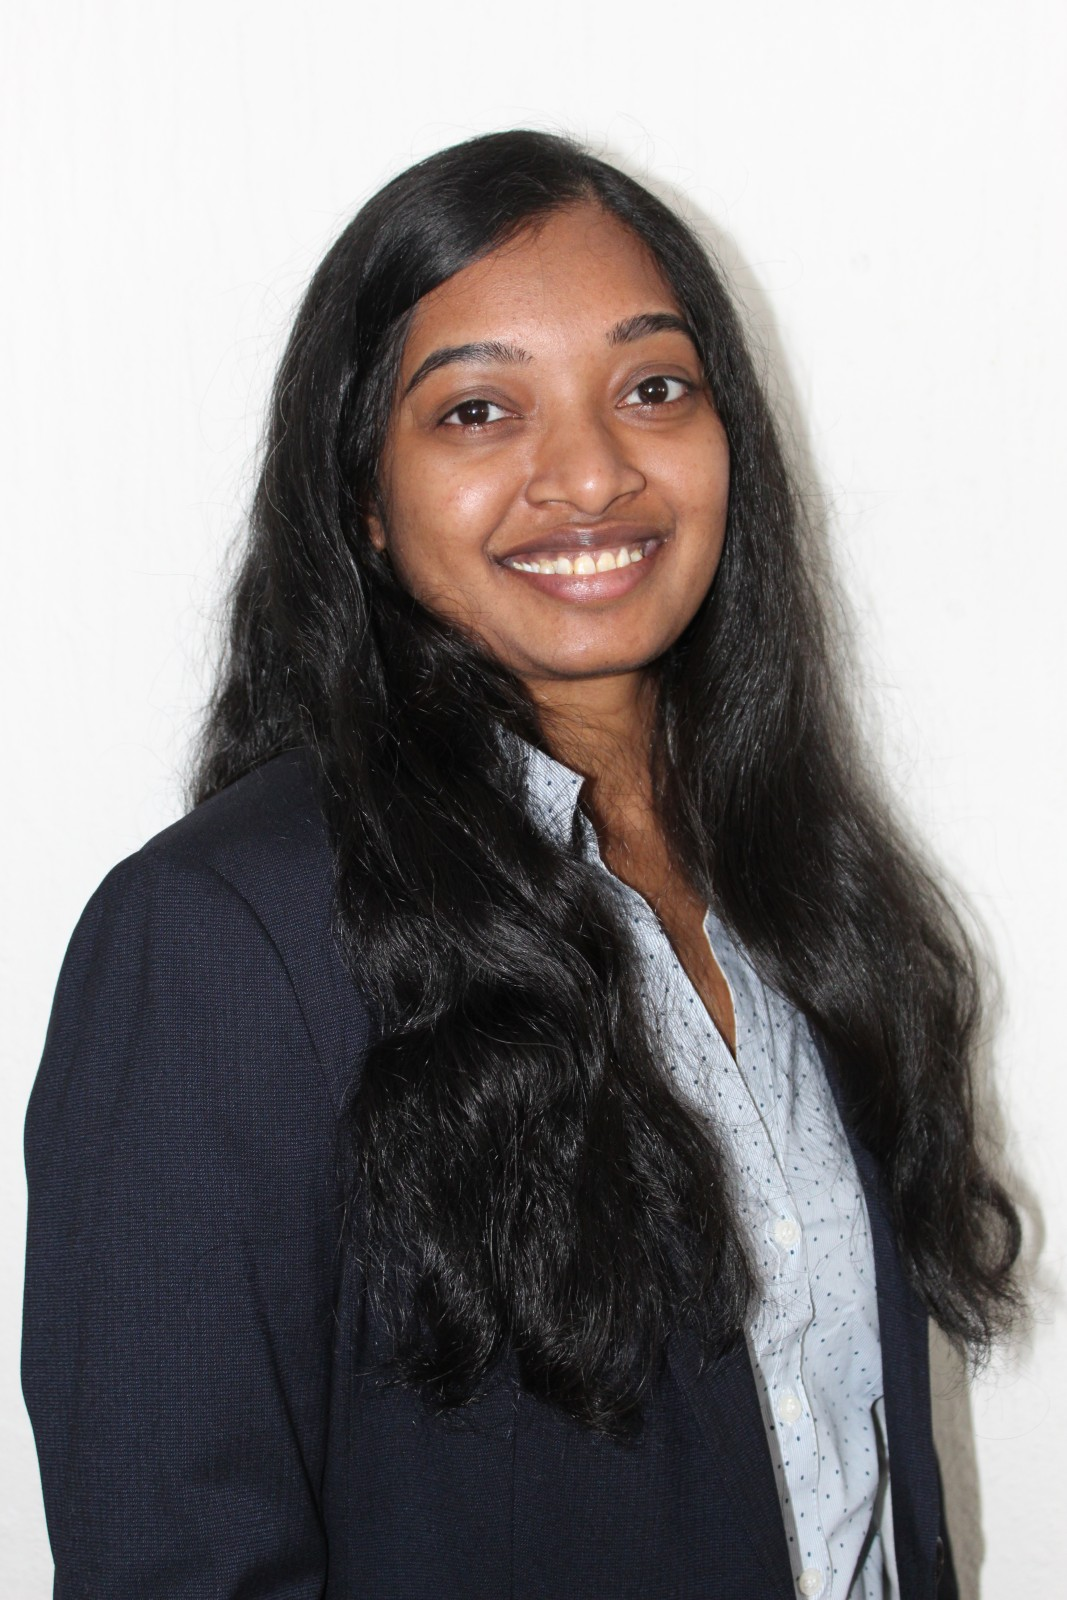
\includegraphics[width=0.3\textwidth]{pic}\par\vspace{3cm}

\section{Pers\"onliche Daten}
\cventry{Anschrift}{\normalfont{Gebersheimer Str. 73}}{}{71229 Leonberg}{}{}
\cventry{Mobil}{\normalfont{+49 152 29 962032}}{}{}{}{}
\cventry{E-Mail}{\href{mailto:shobanamariappan1991@gmail.com}{shobanamariappan1991@gmail.com}}{}{}{}{}
\cventry{Geburtsdatum}{\normalfont{10.03.1991}}{}{}{}{}
\cventry{Familienstand}{\normalfont{verheiratet}}{}{keine Kinder}{}{}
\cventry{Staatsangeh\"origkeit}{\normalfont{Indisch}}{}{}{}{}
\cventry{Portfolio}{\href{https://shobanamariappan.de/}{https://www.shobanamariappan.de/}}{}{}{}{}
\cventry{Github}{\href{https://github.com/shobanaM1991}{https://github.com/shobanaM1991}}{}{}{}{}


%\vspace{5 cm}
%\makecvtitle
\section{T\"atigkeiten}
\subsection{Berufliche Werdegang}
\cventry{Nov 2021--Jetzt}{Testingenieur}{}{\newline Rohde und Schwarz, Weilimdorf, Suttgart}{}
{\textbf{Aufgabe}: Test-case Entwicklung, Testdatengenerierung mit xml on VOIP devices, Test Execution mit Tomcat server, documents update.
}
\cventry{Jan 2021--Oct 2021}{Frontend-entwickler}{}{\newline Mini Projekte}{}
%{\textbf{Full-Stack Entwicklung:} Employee Management Tool: Frontend-React, Backend-Nodejs, DB-MySQL, CRUD Application mit Symfony und Angular CLI \newline
%{\textbf{Frontend-Entwicklung:} Responsive website: HTML5 und CSS3, WordPress Elementor, Ecommerce E-bike website: React und CSS3, Ecommerce E-Learning website: Gatsby und Bootstrap}}
{\textbf{Frontend-Entwicklung:} Responsive website: HTML5 und CSS3, Ecommerce E-bike website: React und CSS3, Ecommerce E-Learning website: Bootstrap \newline
{\textbf{Automatisierungstests-Entwicklung:} UI-Automatisierungstests mit Selenium Python: POM -Konzept mit Unittest Framework, Test-case Entwicklungs, Test Simulation, Report generation mit Bibliothek: HTML Test Runner}}

\cventry{Aug 2019 -- Sep 2020}{Laboringenieurin}{}{\newline GlenDimplex Deutschland GmbH, Kulmbach, Deutschland}{}
{\textbf{Aufgabe}:  Python Programmierung, Data Analytik mit Pandas, NumPy, Seaborn, Frontend-Entwicklung mit TKinter und PyQt5 }

\cventry{M\"ar 2017 -- Aug 2018}{\textbf{Wissenschaftliches Hilfskraft}}{\newline Friedrich-Alexander-Universit\"at}{Erlangen-N\"urnberg}{}
{\textbf{Aufgabe}: Test-case Entwickler, Non-Functional Testing }

\cventry{Jul 2012 -- Sep 2015}{Software-Testingenieur}{}{\newline Accenture Services Private Limited, Chennai,Indien}{}
{\textbf{Aufgabe}: Selenium Automatisierung mit Python, Test-case Entwickler, Qualitätskontrolle
}


\section{Hochschulausbildung}
\cventry{Okt 2015 -- Sep 2018}{Master's Computational Engineering}
%	Erwartetes Abschlussdatum Dez 2017
{\newline Friedrich-Alexander-Universit\"at} {Erlangen-N\"urnberg}{\textit{Abschlussnote -- 2,3}}
{\textbf{Schwerpunkt}: Advanced Programming in C++ and Python, High Performace Computing,
Simulation and Scientific Computing, Supercomputer, Thermo-Fluid Dynamics. }

\cventry{Aug 2008 -- Mai 2012}{Bachelor's Elektrotechnik und Elektronik}{\newline Sona College of Technology}{Salem, Indien}{\textit{Abschlussnote -- 2,3}}
{\textbf{Schwerpunkt}: C ++ Programmierung, Mikroprozessor und Mikrocontroller, Mathmatik, DC und AC-Maschinen, Leistungselektronik, Digitale Logikschaltung.}

\section{Auszeichnungen und Zertifikate}
%\cvitem{2020} {Zertifiziert in Python for Data Science and Machine Learning boot camp in Udamy} 
\cvitem{2022} {Teilnehmer in ISTQB Foundation Level - Udemy}
%\cvitem{2021} {Shopware Template Training (Basic and Advanced), Shopware Developer Training-Basic}
%\cvitem{2021} {Charming Development in Symfony5 from sfcasts}
\cvitem{2021}{Telc - B1, Deutsch- Teilnehmer B2, Deutschland}

\thispagestyle{empty}



\section {IT-Kenntnisse}
\cvitem{Gr\"undkenntnisse}{MySQL, C++}
%\cvitem{Mittlere Kenntnisse}{CSS, PHP, MySQL, WordPress, Visual Studio} , MVC Framework Architecture
\cvitem{Fortgeschrittene Kenntnisse}{C, Python (Numpy, Pandas, Matplotlib, Seaborn, TKinter), HTML5, CSS3, SASS, Bootstrap, JavaScript, Microsoft Office, Linux, \LaTeX}
\cvitem{Tools/Framework Kenntnisse}{JIRA, Git, Visual Studio Code, Selenium, Unittest, Eclipse}
%\cvitem{Framework Kenntnisse}{Selenium, Unittest, Gatsby}
\thispagestyle{empty}

\section{Sprachen}


\cvitem{Tamilisch}{Muttersprache}{}
\cvitem{Englisch}{Fortgeschrittene Kenntnisse - Verhandlungssicher}
\cvitem{Deutsch}{Gute Kenntnisse - B1-Niveau}
\vspace{-0.5cm}


\begin{flushleft}
	\vspace{1\baselineskip}
	\today\\
\includegraphics[width=4cm]{sign_shobana.pdf} \vspace{-1cm}
	
	\vspace{2\baselineskip}
	\textbf{Shobana Mariappan}
\end{flushleft}

\end{document}


%% end of file `template.tex'.
